\section{Управление контуром обратной связи}
\label{sec:Chapter5} \index{Chapter5}

Теоремы главы~\ref{sec:Chapter3} не только объясняют деградацию, но и указывают
точки вмешательства. В этой главе из них выводится критерий риска и проверяется,
какие стратегии формирования выдачи приближают решение
задачи~\eqref{eq:optimal_control}, сохраняя разнообразие без существенной потери
качества.
По смыслу это соответствует линии работ о смягчении эффектов петель обратной связи: вмешательство
может быть каузальным, алгоритмическим или управленческим, но оно должно менять
сам контур, а не только итоговую метрику~\cite{krauth2022,
stoecker2025biasMitigation, pagan2023feedbackLoops}.

\subsection{Точки вмешательства}
\label{subsec:control_targets}

Асимптотическая нижняя грань разнообразия в Теореме~\ref{thm:beta} равна
$\beta\sigma_\xi^2/(2-\beta)$ и пропорциональна разбросу показанного
$\sigma_\xi^2=\operatorname{tr}\Sigma_\xi$. Отсюда прямое следствие: чтобы
удержать разнообразие, нужно не позволять выдаче сужаться, то есть поддерживать
$\sigma_\xi^2$ на ненулевом уровне. Петлевой канал (Теорема~\ref{thm:loop})
действует в противоположную сторону~--- понижает $\sigma_\xi^2$ за счёт роста
резкости $A$, поэтому управление сводится к двум независимым рычагам:
ослаблению загрязнения логов $\alpha=ps$ (оно гасит и петлевой канал, и
завышение наблюдаемых метрик из предложения~\ref{prop:self_reinforcement}) и
прямому расширению выдачи. В терминах теории управления это два разных класса
действий: изменение канала измерения и изменение управляющего сигнала выдачи
~\cite{depasquale2026controlSystems, chandrasekaran2026networkAware}.

Петлевой эффект имеет мультипликативную природу: он возникает лишь при
одновременном выполнении нескольких условий, и достаточно нарушить любое одно из
них, чтобы его обезвредить. Перечень условий и соответствующих управляющих
воздействий сведён в таблице~\ref{tab:checklist}. Такая таблица играет роль
практического контрольного списка, аналогичного таксономическим подходам к классификации
петель обратной связи и способов смягчения смещений~\cite{pagan2023feedbackLoops,
stoecker2025biasMitigation}.

\begin{table}[H]
    \caption{Условия активации петлевого канала и рычаги управления}
    \label{tab:checklist}
    \centering
    \begin{tabular}{p{4.2cm}p{2.4cm}p{6.2cm}}
        \toprule
        Условие & Символ & Рычаг управления \\
        \midrule
        Модель различает пользователей & $\lVert J_k\rVert\neq0$ &
        холодный старт безопаснее; штраф на чувствительность оценки \\
        Аудитория сегментирована & $K\ge2$ &
        контроль однородности сегментов \\
        Логи загрязнены & $\alpha=ps>0$ &
        понижать $p$ или $s$: исследовательские показы, взвешивание навязанных
        откликов \\
        Выдача продолжает сужаться & $\sigma_\xi^2\!\downarrow$ &
        расширение выдачи, контроль резкости $A$ \\
        \bottomrule
    \end{tabular}
\end{table}

\subsection{Сравнение стратегий выдачи}
\label{subsec:interventions}

Чтобы выяснить, какое вмешательство действительно поддерживает разнообразие,
сравнивались пять стратегий формирования списка: жадная top-$L$ (базовая),
$\varepsilon$-жадная при $\varepsilon\in\{0{,}1;0{,}3\}$, softmax с температурой
$\tau=2{,}0$ и стратегия с явным контролем разнообразия по алгоритму максимальной
маргинальной релевантности (MMR). Оценивались сохранение следа ковариации
$\operatorname{tr}\hat\Sigma_T$ и качество выдачи после $T=100$ шагов
(таблица~\ref{tab:h5}, рис.~\ref{fig:h5_trace}). Контроль разнообразия является
классическим направлением в рекомендательных системах~\cite{adomavicius2005}, но
в данной работе он проверяется как управляющее воздействие на долгосрочную
геометрию пользовательских состояний, а не только как одношаговый критерий
качества.

\begin{table}[H]
    \caption{Сравнение стратегий выдачи после $T=100$ шагов (среднее по $3$ запускам)}
    \label{tab:h5}
    \centering
    \begin{tabular}{lrr}
        \toprule
        Стратегия & $\operatorname{tr}\hat\Sigma_T$ & Качество \\
        \midrule
        Базовая (top-$L$)                       & $0{,}289$ & $0{,}634$ \\
        $\varepsilon$-жадная ($\varepsilon{=}0{,}1$) & $0{,}269$ & $0{,}636$ \\
        $\varepsilon$-жадная ($\varepsilon{=}0{,}3$) & $0{,}194$ & $0{,}636$ \\
        softmax ($\tau{=}2{,}0$)                & $0{,}084$ & $0{,}642$ \\
        \textbf{Контроль разнообразия (MMR)}    & $\mathbf{0{,}442}$ & $0{,}641$ \\
        \bottomrule
    \end{tabular}
\end{table}

\begin{figure}[H]
    \centering
    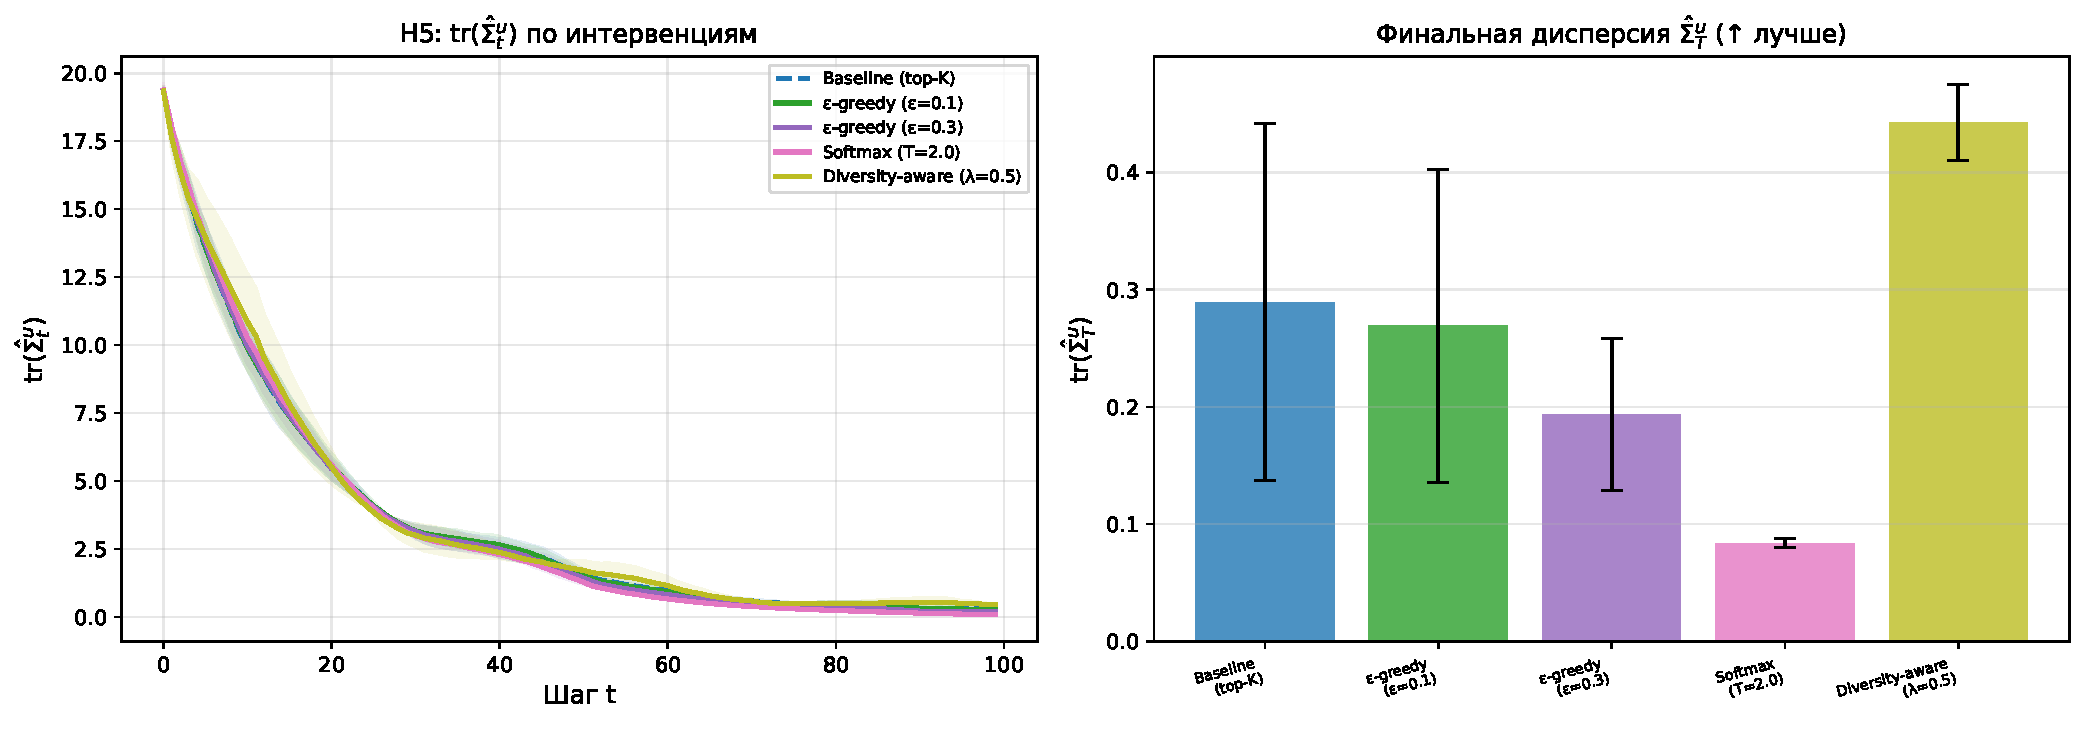
\includegraphics[width=\textwidth]{figures/H5_interventions_trace_sigma}
    \caption{Сохранение следа ковариации $\operatorname{tr}\hat\Sigma_t$ для пяти
    стратегий выдачи. Явный контроль разнообразия (MMR) сохраняет дисперсию выше
    базовой стратегии; случайные стратегии ($\varepsilon$-жадная, softmax)
    усиливают стягивание.}
    \label{fig:h5_trace}
\end{figure}

Результат содержит контринтуитивный вывод. Случайные стратегии~---
$\varepsilon$-жадная и softmax~--- стягивание не ослабляют, а \emph{усиливают}:
случайные показы выводят пользователей на объекты из разных сегментов, в среднем
расположенные ближе к центру пространства, и дрейф~\eqref{eq:drift} стягивает
всю популяцию к единой средней точке быстрее, чем жадная выдача. Напротив,
стратегия с явным контролем разнообразия сохраняет след ковариации
$0{,}442$ против $0{,}289$ у базовой~--- улучшение на $53\%$~--- при практически
том же качестве ($0{,}641$ против $0{,}634$). Механизм согласуется с
разделом~\ref{subsec:control_targets}: MMR штрафует за сходство показанных
объектов, поднимая $\sigma_\xi^2$, а значит и нижнюю грань разнообразия
Теоремы~\ref{thm:beta}. Компромисс качество--разнообразие для всех стратегий
показан на рис.~\ref{fig:h5_pareto}.

\begin{figure}[H]
    \centering
    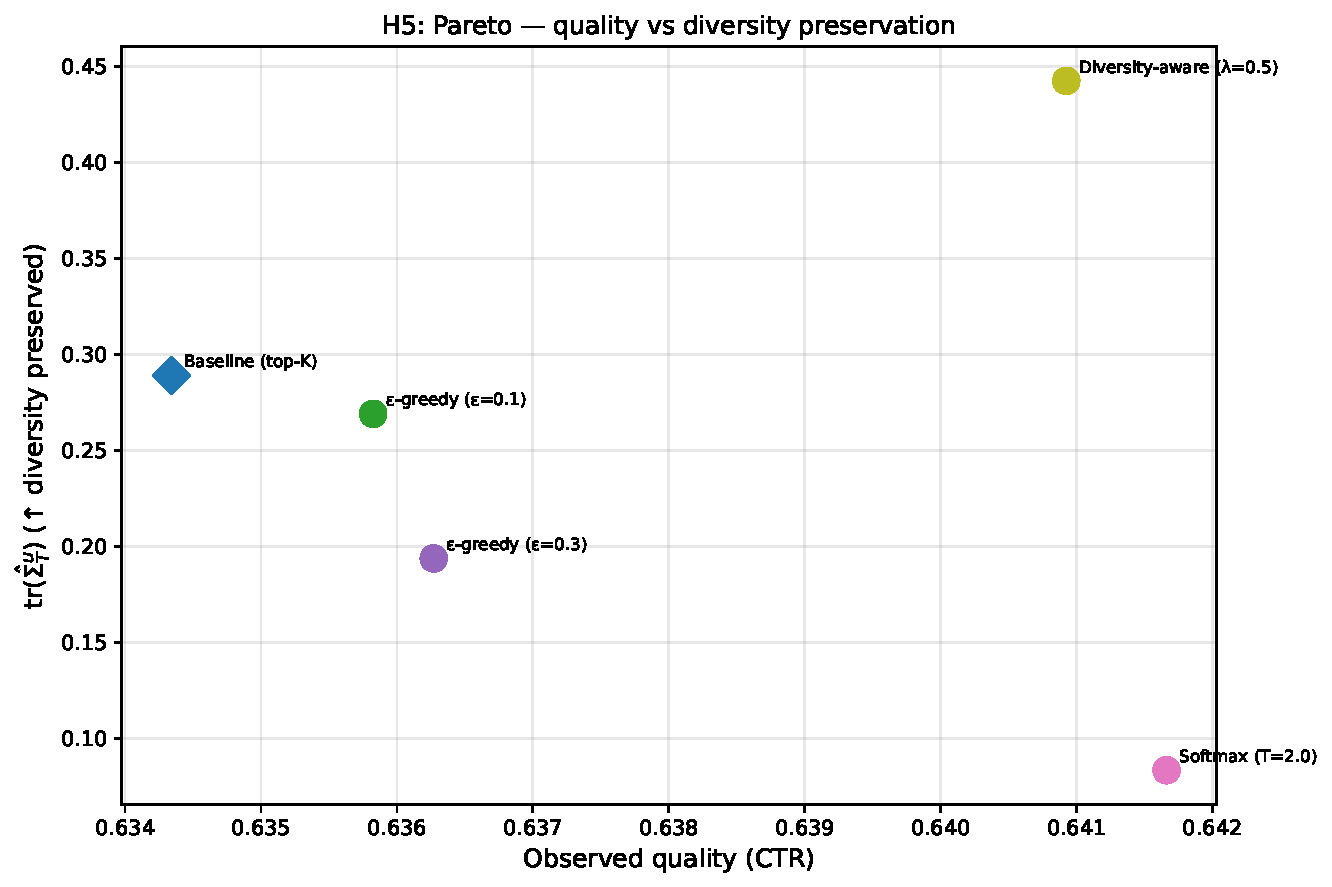
\includegraphics[width=0.8\textwidth]{figures/H5_pareto_quality_diversity}
    \caption{Компромисс между качеством выдачи и сохранением разнообразия для
    пяти стратегий. Стратегия с контролем разнообразия доминирует базовую,
    одновременно сохраняя качество.}
    \label{fig:h5_pareto}
\end{figure}

\textbf{Итог главы.} Управление контуром эффективно тогда, когда оно нацелено на
\emph{форму} выдачи, а не на её случайность. Случайное исследование не защищает
от стягивания и даже ускоряет его; защищает явное расширение выдачи в сочетании
с понижением загрязнения логов $\alpha=ps$. Тем самым на четвёртую задачу
раздела~\ref{subsec:questions} получен конструктивный ответ: предложен критерий
риска (таблица~\ref{tab:checklist}) и подтверждена работоспособность диверсификации
выдачи как меры подавления петлевого канала. В отличие от чисто эвристического
исследования выдачи, такой подход ближе к оптимальному управлению с ограничениями:
качество выдачи
должно оставаться не хуже приемлемого базового уровня, а управляющее воздействие
должно ограничивать накопление долгосрочного риска~\cite{chow2014baselineControl,
mariano2026optimalControl}.
